\documentclass[letterpaper]{article}
\synctex=1
\usepackage{graphicx}
\graphicspath{ {images/} }

\usepackage{lipsum}
\usepackage{float}

% \usepackage[
%     style=ieee,
%     backend=biber
%     ]{biblatex}
% \addbibresource{references.bib}

\usepackage{hyperref}

\usepackage{amssymb}

\usepackage{siunitx}

\usepackage{multirow}
% for merging table cells I think

\usepackage{tabularx}
\renewcommand\tabularxcolumn[1]{m{#1}}% for vertical centering text in X column
% allows for linewrap within cells
\newcolumntype{Y}{>{\centering\arraybackslash}X}

\usepackage{todonotes}
\usepackage{pdfpages}

\usepackage{fancyhdr} %header
\fancyhf{}
\fancyhead[R]{Arun Woosaree XXXXXXX}
\renewcommand\headrulewidth{0pt}
\fancyfoot[C]{\thepage}
\renewcommand\footrulewidth{0pt}
\pagestyle{fancy}

\usepackage[pdf]{graphviz}
\usepackage{adjustbox}

\usepackage{amsmath}
 
% make subsection use letters
\renewcommand{\thesubsection}{\alph{subsection})}


% \usepackage{amsthm}
\title{ECE 322 \\
Assignment 2}
  \author{Arun Woosaree\\
  XXXXXXX} 
%actual document
\begin{document}

\maketitle %insert titlepage here

\section{Credit Union}
\begin{adjustbox}{center}
	\begin{tabular}{lllll}
		Conditions            & \multicolumn{4}{l}{Rules}             \\
		                      & 1                         & 2 & 3 & 4 \\ \cline{2-5}
		city dweller          & 1                         & x & 0 & x \\
		male                  & 1                         & 1 & 0 & 1 \\
		female                & 0                         & 0 & 1 & 0 \\
		age $<25$             & x                         & 1 & 0 & 0 \\
		$25<$ age $<65$       & x                         & 0 & 1 & 0 \\
		age $>65$             & x                         & 0 & 0 & 1 \\
		                      &                           &   &   &   \\
		Actions               &                           &   &   &   \\ \cline{1-1}
		Show Product A        & 1                         & x & x & x \\
		Show Product B        & x                         & 1 & x & x \\
		Show Product C        & x                         & x & 1 & x \\
		Do Not Show Product D & 0                         & 0 & 0 & 1 \\
	\end{tabular}%
\end{adjustbox}
Note: Do Not Show Product D $=0$ means that Product D will be shown.

\subsection{Maximal number of rules}
Given there are 2 possibilities for gender (in this problem), 2 possibilities
for city dweller, and 3 possibilities for age, the maximal number of rules is
$2 \times 2 \times 3 = 12$. 

\subsection{Simplified table}
The table above is already simplified, so here are the resulting test cases:
\vspace{20pt}
\begin{adjustbox}{center}
	\begin{tabular}{ccccccccc}
		Test & city dweller & male & female & age $<25$ & $25<$ age $<65$ & age $>65$ & Expected              \\ \cline{1-1} \cline{8-8}
		1    & 1            & 1    & 0      & 1         & 0               & 0         & Show Product A        \\
		2    & 1            & 1    & 0      & 1         & 0               & 0         & Show Product B        \\
		3    & 0            & 0    & 1      & 0         & 1               & 0         & Show Product C        \\
		4    & 1            & 1    & 0      & 0         & 0               & 1         & Do Not Show Product D \\
	\end{tabular}
	\end{adjustbox} \todo{use a specific age in the test cases}

\section{}
For the given subdomain, the following lines form the boundaries:
\begin{itemize}
	\item $y=5, 0\leq x\leq 7$
	\item $x=0, 0\leq y \leq 5$
	\item $y=-x, 0\leq x\leq 1$
	\item $y=x-2, 1\leq x \leq 7$
\end{itemize}

\subsection{EPC Strategy}
From the boundary lines, we see that the maximum value that $x$ can have is
$7$, its minimum is $-1$, and that the maximum value that $y$ can have is
5 while its minimum value is 0. Using the EPC testing strategy,
$4^2 + 1=17$ test cases are expected. The extreme points chosen are
$(7, 7.1, 0, -0.1)$ for $x$, and $(5, 5.1, 0, -0.1)$ for $y$.
For the additional test case within the boundary, $(x=1, y=1)$ is chosen.
The full list of suggested test cases is found below:


\begin{adjustbox}{center}
	\begin{tabular}{lll}
		test id & x    & y    \\ \hline
		1       & 7    & 5    \\
		2       & 7    & 5.1  \\
		3       & 7    & -1   \\
		4       & 7    & -0.1 \\
		5       & 7.1  & 5    \\
		6       & 7.1  & 5.1  \\
		7       & 7.1  & -1   \\
		8       & 7.1  & -0.1 \\
		9       & 0    & 5    \\
		10      & 0    & 5.1  \\
		11      & 0    & -1   \\
		12      & 0    & -0.1 \\
		13      & -0.1 & 5    \\
		14      & -0.1 & 5.1  \\
		15      & -0.1 & -1   \\
		16      & -0.1 & -0.1 \\
		17      & 1    & 1    \\
	\end{tabular}
\end{adjustbox}

\subsection{Weak n x 1 Strategy}
Given that there are 4 boundaries, we expect $4(2+1) +1 = 13$ test cases.
The dimensionality is 2, so 2 points are chosen on each boundary, as well
as one additional point just outside of each boundary. The last test case
is one point inside the boundaries. The full list of suggested test cases
is found below:

\begin{adjustbox}{center}
	\begin{tabular}{llll}
		test id & description                              & x    & y    \\ \hline
		1       & on $y=5, 0\leq x\leq 7$ boundary         & 2    & 5    \\
		2       & on $y=5, 0\leq x\leq 7$ boundary         & 4    & 5    \\
		3       & outside $y=5, 0\leq x\leq 7$ boundary    & 3    & 5.1  \\
		4       & on $x=0, 0\leq y \leq 5$ boundary        & 0    & 2    \\
		5       & on $x=0, 0\leq y \leq 5$ boundary        & 0    & 4    \\
		6       & outside $x=0, 0\leq y \leq 5$ boundary   & -0.1 & 3    \\
		7       & on $y=-x, 0\leq x\leq 1$ boundary        & 0.3  & -0.3 \\
		8       & on $y=-x, 0\leq x\leq 1$ boundary        & 0.7  & -0.7 \\
		9       & outside  $y=-x, 0\leq x\leq 1$ boundary  & 0.5  & -0.6 \\
		10      & on $y=x-2, 1\leq x \leq 7$ boundary      & 3    & 1    \\
		11      & on $y=x-2, 1\leq x \leq 7$ boundary      & 5    & 3    \\
		12      & outside $y=x-2, 1\leq x \leq 7$ boundary & 4    & 1.9  \\
		13      & Inside the boundaries                    & 1    & 1    \\
	\end{tabular}
\end{adjustbox}

\section{Cause-Effect Graph}
From the following decision table, the cause effect graph below is generated:

\begin{adjustbox}{center}
	\begin{tabular}{llllllllllll}
		Conditions         &   &   &   &   &   &   &   &   &   &   &   \\ \cline{1-1}
		C1: $a<b+c$?       & 0 & 1 & 1 & 1 & 1 & 1 & 1 & 1 & 1 & 1 & 1 \\
		C2: $b<a+c$?       & x & 0 & 1 & 1 & 1 & 1 & 1 & 1 & 1 & 1 & 1 \\
		C3: $c<a+b$?       & x & x & 0 & 1 & 1 & 1 & 1 & 1 & 1 & 1 & 1 \\
		C4: $a=b$?         & x & x & x & 1 & 1 & 1 & 1 & 0 & 0 & 0 & 0 \\
		C5: $a=c$?         & x & x & x & 1 & 1 & 0 & 0 & 1 & 1 & 0 & 0 \\
		C6: $b=c$?         & x & x & x & 1 & 0 & 1 & 0 & 1 & 0 & 1 & 0 \\
		                   &   &   &   &   &   &   &   &   &   &   &   \\
		Actions            &   &   &   &   &   &   &   &   &   &   &   \\ \cline{1-1}
		A1: Not a Triangle & 1 & 1 & 1 & x & x & x & x & x & x & x & x \\
		A2: Scalene        & x & x & x & x & x & x & x & x & x & x & 1 \\
		A3: Isosceles      & x & x & x & x & x & x & 1 & x & 1 & 1 & x \\
		A3: Equilateral    & x & x & x & 1 & x & x & x & x & x & x & x \\
		A4: Impossible     & x & x & x & x & 1 & 1 & x & 1 & x & x & x \\
	\end{tabular}
\end{adjustbox}
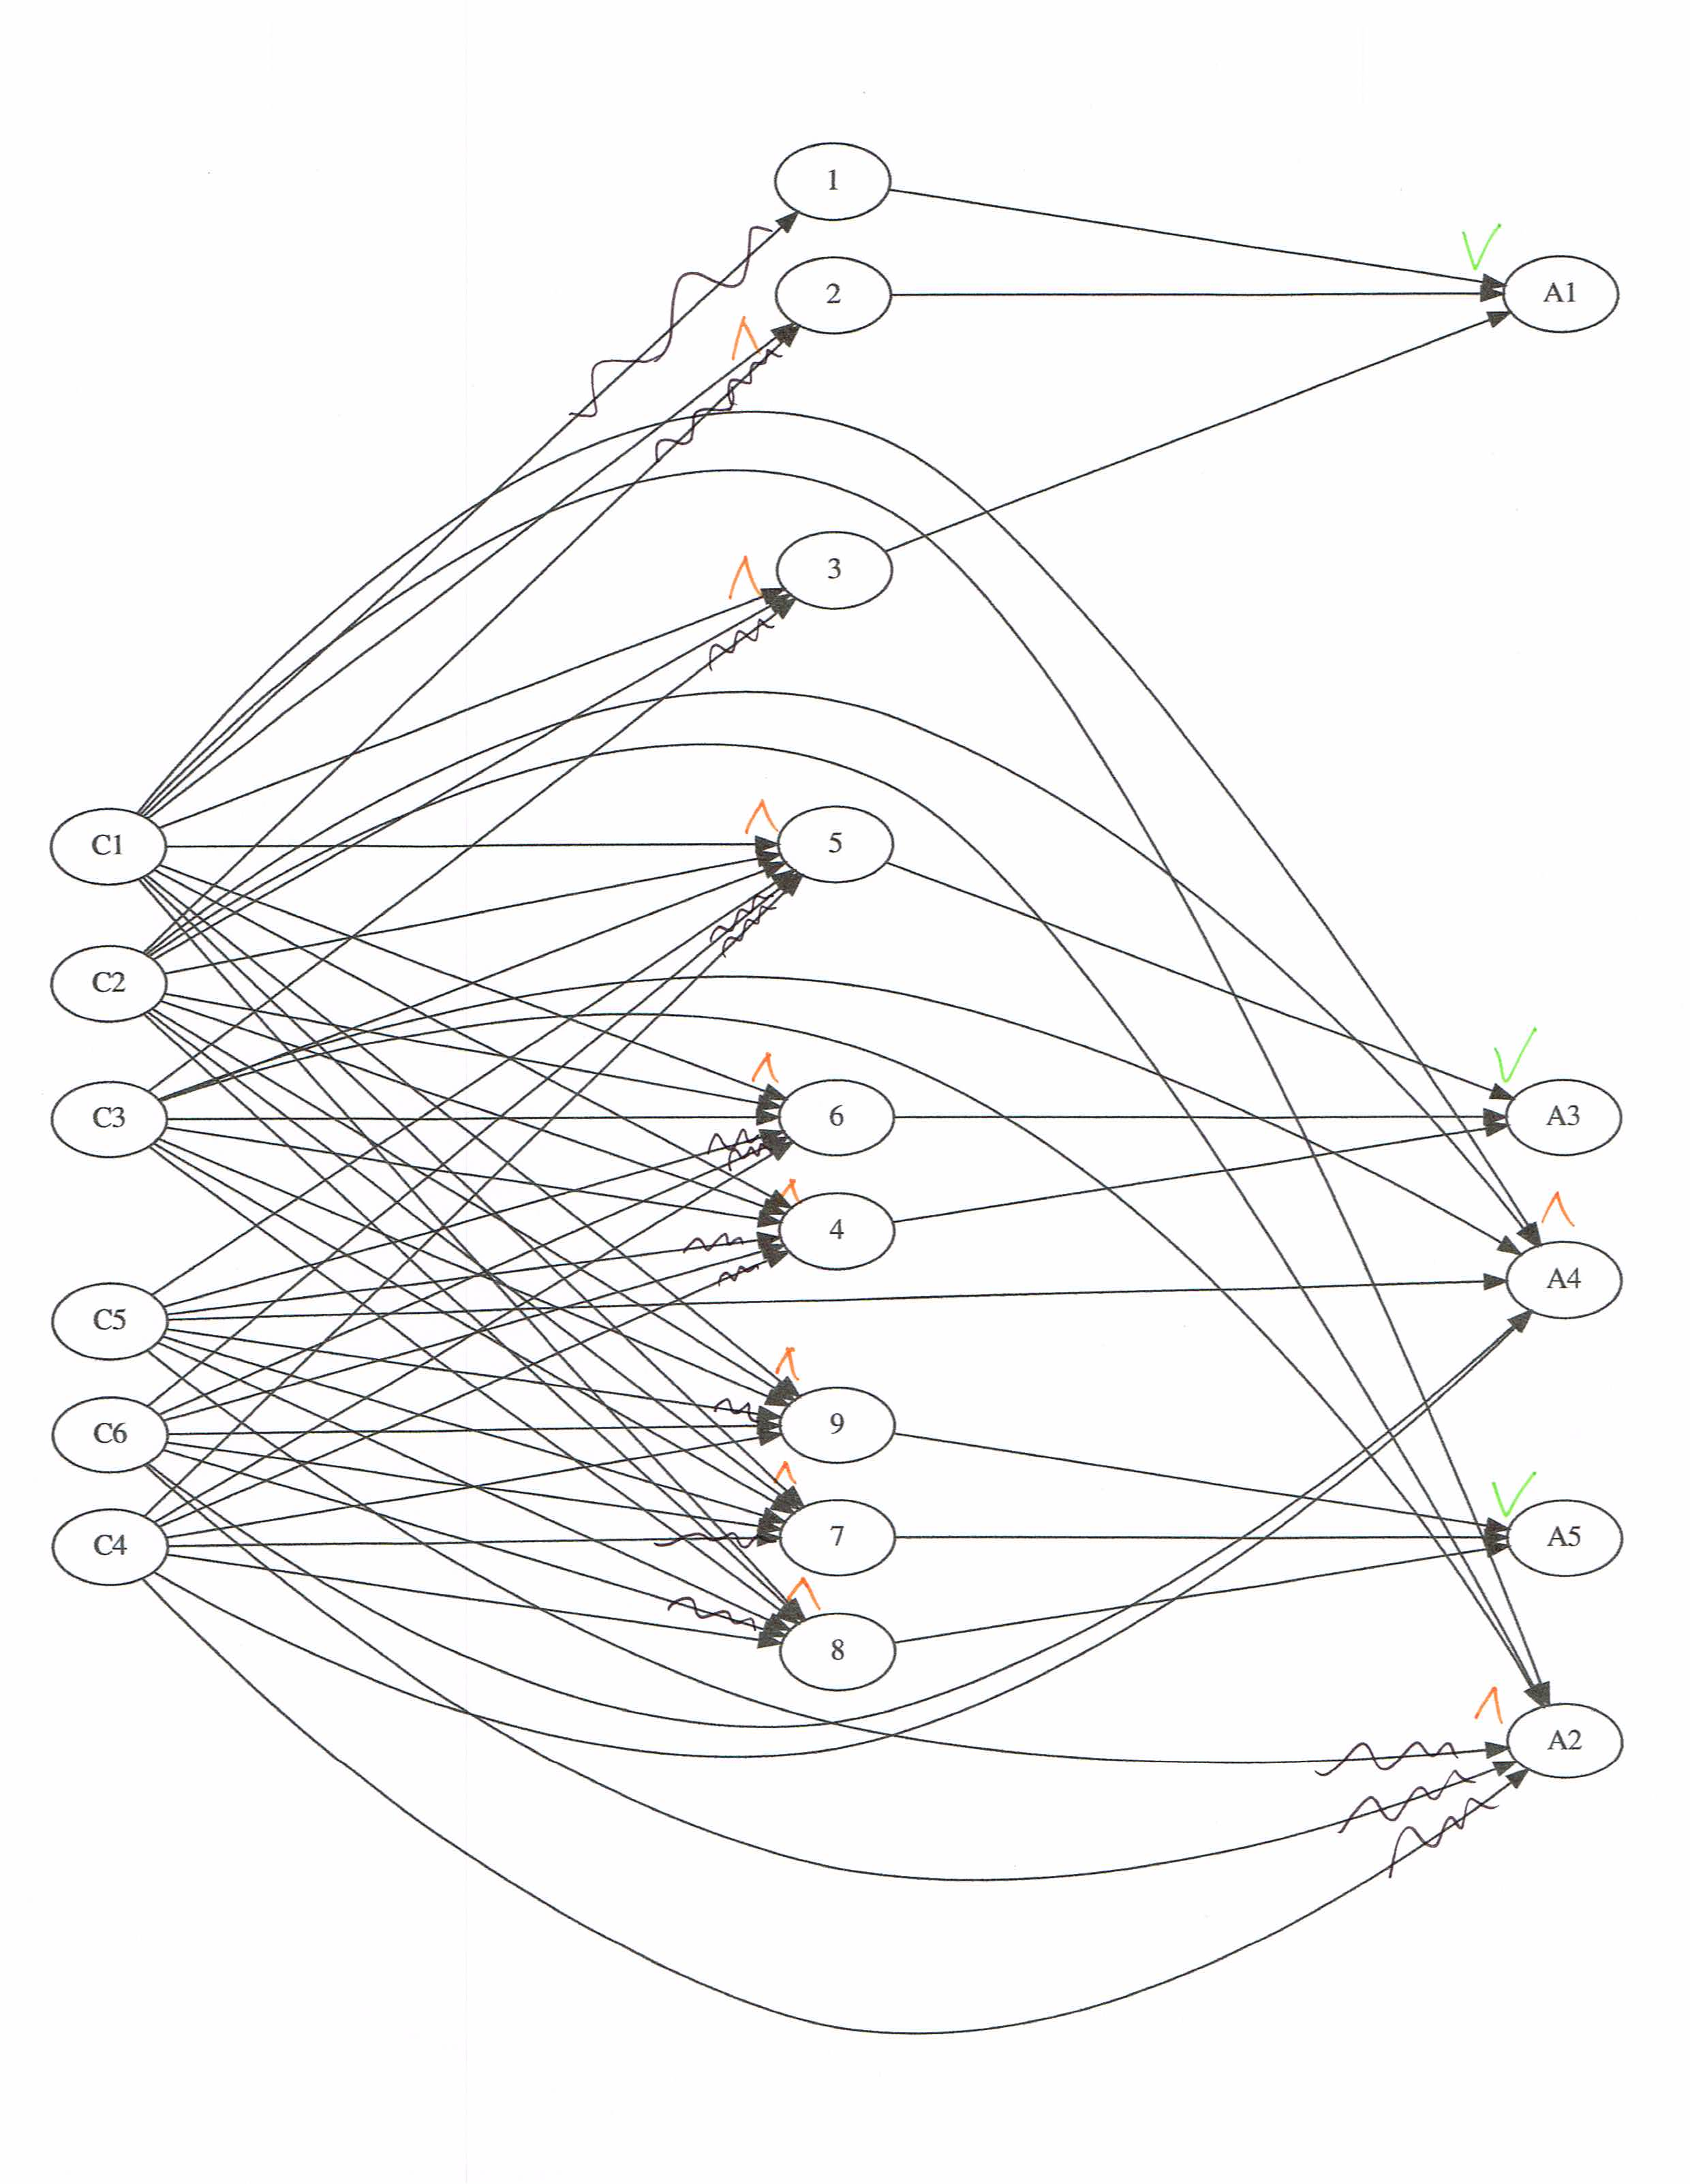
\includepdf{causeeffect.jpg}

\section{Test Cases}
The following description table is derived from the cause effect graph
(Because of the requires, $(C3=1, C6=0)$ will never happen)
\vspace{20pt}
\begin{adjustbox}{center}
	\begin{tabular}{llllll}
		           & 1 & 2 & 3 & 4 & 5 \\ \cline{2-6}
		Conditions &   &   &   &   &   \\ \cline{1-1}
		C3         & 1 & 0 & 0 & x & 0 \\
		C4         & x & x & 1 & x & 0 \\
		C5         & 1 & x & 1 & 0 & x \\
		C6         & 1 & 0 & 1 & x & x \\
		           &   &   &   &   &   \\
		Effects    &   &   &   &   &   \\ \cline{1-1}
		E          & 1 & 0 & 1 & 0 & 0 \\
	\end{tabular}
\end{adjustbox}
\vspace{20pt}

From the decision table above, the following test cases are generated:
\vspace{20pt}

\begin{adjustbox}{max width=\textwidth, center}
	\begin{tabular}{llllll}
		Test & C3 & C4 & C5 & C6 & Expected \\ \cline{1-1} \cline{6-6}
		1    & 1  & 0  & 1  & 1  & 1        \\
		2    & 0  & 1  & 1  & 0  & 0        \\
		3    & 0  & 1  & 1  & 1  & 1        \\
		4    & 1  & 1  & 0  & 1  & 0        \\
		5    & 0  & 0  & 1  & 1  & 0        \\
	\end{tabular}
\end{adjustbox}
\section{Combinatorial Testing}
There are
$2 \times 3 \times 3 \times 3 \times 3 \times 2 \times 3 \times 3 = 2916$
total possible combinations to test.
Ideally, the orthogonal array should be $2^2 3^6$,
resulting in

some fucking magic later: \todo{\#todo: explain}


The following mapping is created:
\vspace{20pt}
\begin{adjustbox}{max width=1.5\textwidth, center}
	\begin{tabular}{ccccccccc}
		   & PRINTERS & PLUGINS & BROWSERS & OPERATING SYSTEMS & SERVERS & MONITORS & EMAIL SYSTEMS & SOFTWARE PACKAGES \\
		1  & printer2 & plugin2 & browser3 & os1               & server2 & monitor2 & email1        & software2         \\
		2  & printer1 & plugin1 & browser1 & os3               & server1 & monitor1 & email2        & software2         \\
		3  & printer1 & plugin2 & browser1 & os2               & server3 & monitor2 & email3        & software1         \\
		4  & printer2 & plugin1 & browser2 & os2               & server2 & monitor1 & email1        & software3         \\
		5  & printer2 & plugin2 & browser2 & os3               & server3 & monitor2 & email2        & software3         \\
		6  & printer1 & plugin1 & browser3 & os1               & server1 & monitor1 & email3        & software3         \\
		7  & printer2 & plugin2 & browser3 & os2               & server1 & monitor1 & email2        & software1         \\
		8  & printer1 & plugin1 & browser2 & os3               & server2 & monitor2 & email3        & software1         \\
		9  & printer1 & plugin1 & browser3 & os3               & server3 & monitor1 & email1        & software2         \\
		10 & printer2 & plugin1 & browser1 & os1               & server1 & monitor2 & email1        & software1         \\
		11 & printer2 & plugin1 & browser2 & os2               & server1 & monitor2 & email3        & software2         \\
		12 & printer1 & plugin1 & browser2 & os1               & server3 & monitor1 & email2        & software3         \\
		13 & printer1 & plugin2 & browser1 & os2               & server2 & monitor2 & email2        & software3
	\end{tabular}%
\end{adjustbox}
\\

resulting in 13 test cases, as opposed to 2916 if we were to test all possible
combinations, a huge improvement.
\end{document}
